\section*{Informations générales}
 
\begin{table}[H]
\centering
	\begin{tabularx}{16.8cm}{|X|X|}
	\hline
	\rowcolor{gray!40} Numéro du risque & Type du risque \\
	\hline
	007 & Perte de documents \\
	\hline
	\end{tabularx}
\end{table}

\begin{table}[H]
\centering
	\begin{tabularx}{16.8cm}{|X|X|X|}
	\hline
	\rowcolor{gray!40} Date & Visa du \RQ & Visa du \CP \\
	\hline
	 28/01/2016 & pgpic & pgpic \\
	\hline
	\end{tabularx}
\end{table}

\begin{table}[H]
\centering
	\begin{tabularx}{16.8cm}{|X|X|X|X|}
	\hline
	\rowcolor{gray!40} Pilote & Activité WBS & Compte WBS & Phase d'apparition \\
	\hline
	 \Mathieu & Suivre les Risques et Opportunités & 1.2.3.2 & À partir du début du projet\\
	\hline
	\end{tabularx}
\end{table}

\section*{Description du risque}

\subsection*{Résumé}
	Le risque lié à la perte de documents peut entrainer une perte du travail réalisé et donc une perte de temps sur l'avancement du projet.
	
\subsection*{Analyse des causes}
	voir figure \ref{risque perte de document}.

\subsection*{Criticité}

\begin{table}[H]
\centering
	\begin{tabularx}{16.8cm}{|>{\columncolor{gray!40}}X|X|}
	\hline
	Gravité & 4\\
	\hline
	Probabilité & 1\\
	\hline
	Criticité & Critique\\
	\hline
	\end{tabularx}
\end{table}
\newpage

\section*{Actions}
\subsection*{Actions préventives}

\centering
	\begin{longtable}{|p{7cm}|p{7cm}|}
	\hline
	\rowcolor{gray!40} Numéro de cause & Actions préventives \\
	\hline
	1 & \begin{itemize}
		\item Formation des membres de l'équipe aux outils
		\end{itemize} \\
	\hline
	2 & \begin{itemize}
		\item Vérification du travail du \RGC{} par le \CP
		\item Vérification du nommage et de l'archivage par le \RGC{} toutes les semaines
		\end{itemize} \\
	\hline
	3 & \begin{itemize}
		\item Formation du \RGC
		\end{itemize} \\
	\hline
	4 & \begin{itemize}
		\item Faire un clone de l'archive toutes les semaines
	\end{itemize} \\
	\hline
	\end{longtable}

\flushleft
\subsection*{Plan de contournement}

\begin{enumerate}
	\item Récupérer la version du document la plus récente possible
	\item Ré-imprimer le document et le refaire valider si besoin
	\item Refaire le travail perdu le plus vite possible
\end{enumerate}

\section*{Décision de clôture}
Par le \CP{} et le pilote du risque.
\begin{table}[H]
\centering
	\begin{tabularx}{16.8cm}{|X|X|}
	\hline
	\rowcolor{gray!40} Date de clôture & Raison de la clôture \\
	\hline
	  & \\
	\hline
	\end{tabularx}
\end{table}

\section*{Historique des modifications}
\begin{table}[H]
\centering
	\begin{tabularx}{16.8cm}{|X|X|}
	\hline
	Date & Modification \\
	\hline
	  & \\
	\hline
	\end{tabularx}
\end{table}
\newpage

\begin{figure}
	\centering
	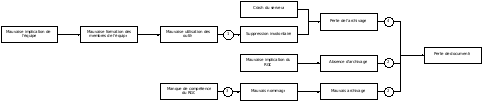
\includegraphics[scale=1, angle=90]{images/AnalyseRisque_nPourquoi_FDR007}
	\caption{\label{risque perte de document}risque perte de document - méthode des n pourquoi}
\end{figure}
